\documentclass[aspectratio=169]{beamer}
\usetheme{SimpleDarkBlue}
\usecolortheme{default}
\usepackage[utf8]{inputenc}
\usepackage{graphicx}
\usepackage{amsmath}
\usepackage{xcolor}
\usepackage{booktabs}
\usepackage{listings}
\usepackage{tikz}
\usetikzlibrary{arrows,shapes,positioning,shadows,trees}

\definecolor{myblue}{RGB}{0,102,204}
\definecolor{myred}{RGB}{204,0,0}
\definecolor{mygreen}{RGB}{0,153,0}

\title{Wykład 2: Komponenty i Architektura Systemów Rozproszonych}
\author{mgr inż. Jakub Woźniak}
\institute{Instytut Informatyki Politechniki Poznańskiej}
\date{}

\begin{document}

% Strona tytułowa
\begin{frame}
    \titlepage
\end{frame}

% Spis treści
\begin{frame}{Plan wykładu}
    \tableofcontents
\end{frame}

\section{Wprowadzenie do systemów rozproszonych}

\begin{frame}{Definicja systemu rozproszonego}
    \begin{block}{Czym jest system rozproszony?}
        System rozproszony to zbiór niezależnych urządzeń technicznych połączonych w jedną, spójną logicznie całość.
    \end{block}
    
    \begin{quote}
        \small ``A distributed system is one in which the failure of a computer you didn't even know existed can render your own computer unusable'' --- Leslie Lamport
    \end{quote}
    
    \vspace{0.5cm}
    
    \begin{itemize}
        \item Obecnie właściwie wszystkie systemy (poza domowymi komputerami) są rozproszone
        \item Ogromnym katalizatorem rozproszenia systemów jest Internet
    \end{itemize}
\end{frame}

\begin{frame}{Kluczowe cechy systemów rozproszonych}
    \begin{columns}
        \begin{column}{0.5\textwidth}
            \begin{itemize}
                \item \textbf{Współdzielenie zasobów}
                \begin{itemize}
                    \small
                    \item Sprzęt, oprogramowanie, dane
                    \item Np. współdzielenie drukarki
                \end{itemize}
                \vspace{0.2cm}
                \item \textbf{Współbieżność}
                \begin{itemize}
                    \small
                    \item Jednoczesne przetwarzanie zadań
                    \item Zwiększa wydajność całego systemu
                \end{itemize}
            \end{itemize}
        \end{column}
        \begin{column}{0.5\textwidth}
            \begin{itemize}
                \item \textbf{Skalowalność}
                \begin{itemize}
                    \small
                    \item Możliwość rozwoju bez wpływu na wydajność
                    \item Dodawanie nowych zasobów w razie potrzeby
                \end{itemize}
                \vspace{0.2cm}
                \item \textbf{Niezawodność}
                \begin{itemize}
                    \small
                    \item Awaria jednego węzła nie powoduje awarii systemu
                    \item Redundancja komponentów
                \end{itemize}
            \end{itemize}
        \end{column}
    \end{columns}
    \vspace{0.3cm}
    \begin{block}{Przejrzystość}
        Tworzenie wrażenia pojedynczego, zintegrowanego systemu, mimo że składa się z wielu niezależnych komponentów.
    \end{block}
\end{frame}

\section{Warstwy systemu}

\begin{frame}{Architektura trójwarstwowa}
    \begin{center}
        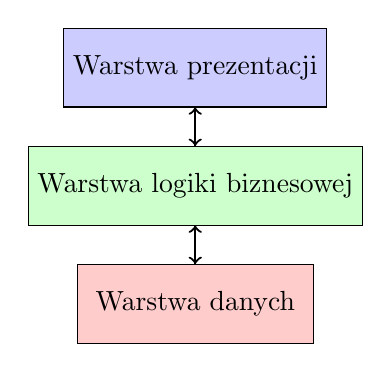
\begin{tikzpicture}[node distance=1.5cm]
            \node (pres) [draw, fill=blue!20, minimum width=3cm, minimum height=1cm] {Warstwa prezentacji};
            \node (logic) [draw, fill=green!20, minimum width=3cm, minimum height=1cm, below of=pres] {Warstwa logiki biznesowej};
            \node (data) [draw, fill=red!20, minimum width=3cm, minimum height=1cm, below of=logic] {Warstwa danych};
            
            \draw[->, thick] (pres) -- (logic);
            \draw[->, thick] (logic) -- (data);
            \draw[->, thick] (logic) -- (pres);
            \draw[->, thick] (data) -- (logic);
        \end{tikzpicture}
    \end{center}
    

    
    \begin{itemize}
        \item Separacja odpowiedzialności
        \item Modularność i możliwość ponownego użycia komponentów
        \item Łatwiejsze testowanie i konserwacja
        \item Możliwość niezależnego skalowania warstw
    \end{itemize}
    \begin{block}{Dyskusja}
        Gdzie Netflix łączy strumienie audio i wideo?
    \end{block}
\end{frame}

\begin{frame}{Warstwa prezentacji}
    \begin{block}{Definicja}
        Interfejs między systemem a użytkownikiem końcowym.
    \end{block}
    
    \begin{itemize}
        \item Odpowiada za:
        \begin{itemize}
            \item Renderowanie danych w formie czytelnej dla użytkownika
            \item Walidację danych wprowadzanych przez użytkownika
            \item Obsługę interakcji użytkownika z systemem
            \item Komunikację z warstwą logiki biznesowej
        \end{itemize}
        \vspace{0.3cm}
        \item W nowoczesnych systemach rozproszonych:
        \begin{itemize}
            \item Aplikacje webowe wykorzystujące cienkich klientów
            \item \textit{Software as a Service} (SaaS)
            \item Klientem jest przeglądarka internetowa
        \end{itemize}
    \end{itemize}
\end{frame}

\begin{frame}{Warstwa logiki biznesowej}
    \begin{block}{Definicja}
        Warstwa odpowiedzialna za implementację reguł biznesowych i logiki, które determinują działanie aplikacji.
    \end{block}
    
    \begin{itemize}
        \item Komponenty:
        \begin{itemize}
            \item \textbf{Encje} - obiekty reprezentujące dane
            \item \textbf{Logika biznesowa} - implementacja reguł biznesowych
            \item \textbf{Dostęp do danych} - komponenty do interakcji z bazą danych
        \end{itemize}
        \vspace{0.3cm}
        \item Korzyści:
        \begin{itemize}
            \item Modułowość
            \item Możliwość ponownego użycia
            \item Testowalność
            \item Skalowalność
        \end{itemize}
    \end{itemize}
\end{frame}

\begin{frame}{Warstwa danych}
    \begin{block}{Definicja}
        Warstwa odpowiedzialna za przechowywanie i dostęp do danych w systemie rozproszonym.
    \end{block}
    
    \begin{itemize}
        \item Komponenty:
        \begin{itemize}
            \item Bazy danych (relacyjne, NoSQL, czasowe)
            \item Systemy plików (lokalne, rozproszone)
            \item Mechanizmy cache'owania
        \end{itemize}
        \vspace{0.3cm}
        \item Kluczowe aspekty:
        \begin{itemize}
            \item Trwałość danych
            \item Spójność danych
            \item Wydajny dostęp do danych
            \item Skalowalność
        \end{itemize}
    \end{itemize}
\end{frame}

\section{Wzorce komunikacji}


\begin{frame}{Komunikacja synchroniczna - HTTP/REST}
    \begin{block}{REST (Representational State Transfer)}
        Styl architektury oprogramowania wykorzystujący protokół HTTP do komunikacji.
    \end{block}
    
    \begin{itemize}
        \item Charakterystyka:
        \begin{itemize}
            \item Wykorzystuje standardowe metody HTTP (GET, POST, PUT, DELETE)
            \item Zazwyczaj używa formatu JSON lub XML
            \item Luźna specyfikacja - "każdy protokół HTTP jest prawidłowy"
            \item Opcjonalnie dokumentacja OpenAPI/Swagger
        \end{itemize}
        \vspace{0.3cm}
        \item Zalety:
        \begin{itemize}
            \item Prostota implementacji
            \item Szeroka obsługa w przeglądarkach
            \item Brak specjalnych bibliotek klienckich
            \item Dobra dokumentacja i narzędzia
        \end{itemize}
    \end{itemize}
\end{frame}

\begin{frame}{Komunikacja synchroniczna - gRPC}
    \begin{block}{gRPC (Google Remote Procedure Call)}
        Nowoczesny framework RPC oparty na HTTP/2 i Protocol Buffers.
    \end{block}
    
    \begin{itemize}
        \item Charakterystyka:
        \begin{itemize}
            \item Wykorzystuje Protocol Buffers (Protobuf) do serializacji
            \item Wymaga ścisłej definicji kontraktu w pliku .proto
            \item Wsparcie dla przesyłania strumieniowego
            \item Automatyczne generowanie kodu klienta
        \end{itemize}
        \vspace{0.3cm}
        \item Zalety:
        \begin{itemize}
            \item Wysoka wydajność
            \item Mały rozmiar przesyłanych danych
            \item Ścisła specyfikacja interfejsu
            \item Wsparcie dla wielu języków programowania
        \end{itemize}
    \end{itemize}
\end{frame}

\begin{frame}{Porównanie HTTP/REST i gRPC}
    \begin{table}
        \begin{tabular}{l|l|l}
            \toprule
            \textbf{Cecha} & \textbf{HTTP/REST} & \textbf{gRPC} \\
            \midrule
            Format & JSON/XML & Protocol Buffers \\
            Protokół & HTTP 1.1 & HTTP/2 \\
            Kontrakt & Opcjonalny (OpenAPI) & Wymagany (.proto) \\
            Streaming & Ograniczony & Pełne wsparcie \\
            Generowanie kodu & Nie & Tak \\
            Wsparcie przeglądarek & Pełne & Ograniczone \\
            Krzywa uczenia & Niska & Średnia \\
            \bottomrule
        \end{tabular}
    \end{table}
\end{frame}

\begin{frame}{Komunikacja synchroniczna - GraphQL}
    \begin{block}{GraphQL}
        Język zapytań i platforma do manipulacji danymi opracowany przez Facebooka w 2015 roku, oferujący alternatywę dla REST.
    \end{block}
    
    \begin{columns}
        \begin{column}{0.5\textwidth}
            \textbf{Główne cechy:}
            \begin{itemize}
                \item Pojedynczy endpoint zamiast wielu endpointów REST
                \item Klient precyzyjnie określa, jakie dane chce otrzymać
                \item Ścisła typizacja dzięki schematowi GraphQL
                \item Introspection - możliwość badania schematu API
            \end{itemize}
        \end{column}
        
        \begin{column}{0.5\textwidth}
            \textbf{Zalety:}
            \begin{itemize}
                \item Eliminacja under/over-fetchingu danych
                \item Łatwiejsza ewolucja API
                \item Zmniejszenie liczby zapytań sieciowych
                \item Silne wsparcie dla dokumentacji
                \item Elastyczne pobieranie powiązanych danych
            \end{itemize}
        \end{column}
    \end{columns}
\end{frame}
\begin{frame}{Komunikacja synchronicznia - GraphQL - cont.}
    
    \begin{center}
        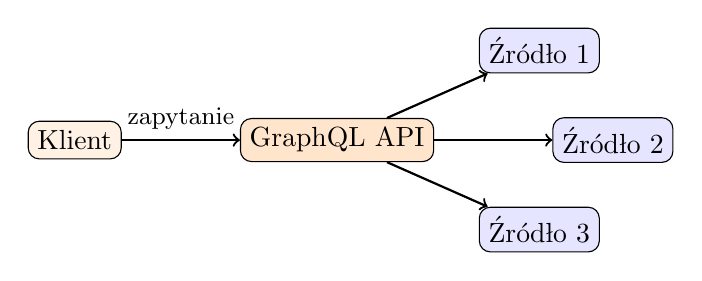
\begin{tikzpicture}[node distance=1.5cm]
            \node[draw, rounded corners, fill=orange!10] (client) {Klient};
            \node[draw, rounded corners, fill=orange!20, right=of client] (graphql) {GraphQL API};
            \node[draw, rounded corners, fill=blue!10, above right=0.8cm of graphql] (source1) {Źródło 1};
            \node[draw, rounded corners, fill=blue!10, right=of graphql] (source2) {Źródło 2};
            \node[draw, rounded corners, fill=blue!10, below right=0.8cm of graphql] (source3) {Źródło 3};
            
            \draw[->, thick] (client) -- (graphql) node[midway, above] {\small zapytanie};
            \draw[->, thick] (graphql) -- (source1);
            \draw[->, thick] (graphql) -- (source2);
            \draw[->, thick] (graphql) -- (source3);
        \end{tikzpicture}
    \end{center}
\end{frame}


\begin{frame}{Komunikacja asynchroniczna - Kolejki wiadomości}
    \begin{block}{Model Point-to-Point}
        Wiadomość wysłana przez nadawcę jest odbierana tylko przez jednego odbiorcę.
    \end{block}
    
    \begin{center}
        
\begin{tikzpicture}
            \node[draw, rounded corners] (sender) at (-3,0) {Nadawca};
            \node[draw, fill=yellow!20, minimum width=4cm, minimum height=1cm] (queue) at (0,0) {Kolejka wiadomości};
            \node[draw, rounded corners] (receiver) at (3,0) {Odbiorca};
            
            \draw[->, thick] (sender) -- (queue);
            \draw[->, thick] (queue) -- (receiver);
        \end{tikzpicture}
    \end{center}
    
    \begin{itemize}
        \item Zalety:
        \begin{itemize}
            \item Izolacja komponentów systemu
            \item Buforowanie wiadomości
            \item Równoważenie obciążenia
            \item Odporność na awarie
        \end{itemize}
    \end{itemize}
    
    \begin{block}{Przykłady implementacji}
        RabbitMQ, Apache Kafka, Amazon SQS
    \end{block}
\end{frame}

\begin{frame}{Komunikacja asynchroniczna - Publish/Subscribe}
    \begin{block}{Model Publish/Subscribe (Pub/Sub)}
        Nadawca publikuje wiadomość na topic, a każdy subskrybent tego topica otrzymuje kopię wiadomości.
    \end{block}
    
    \begin{center}
        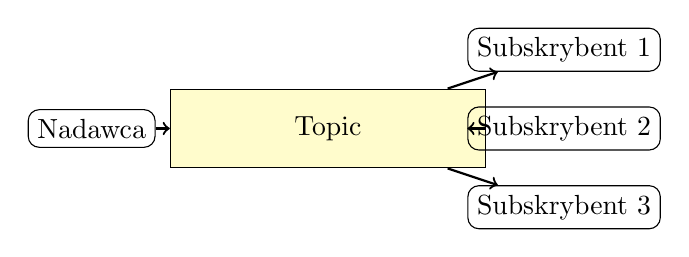
\begin{tikzpicture}
            \node[draw, rounded corners] (publisher) at (-3,0) {Nadawca};
            \node[draw, fill=yellow!20, minimum width=4cm, minimum height=1cm] (topic) at (0,0) {Topic};
            \node[draw, rounded corners] (sub1) at (3,1) {Subskrybent 1};
            \node[draw, rounded corners] (sub2) at (3,0) {Subskrybent 2};
            \node[draw, rounded corners] (sub3) at (3,-1) {Subskrybent 3};
            
            \draw[->, thick] (publisher) -- (topic);
            \draw[->, thick] (topic) -- (sub1);
            \draw[->, thick] (topic) -- (sub2);
            \draw[->, thick] (topic) -- (sub3);
        \end{tikzpicture}
    \end{center}
    
    \begin{itemize}
        \item Główna cecha:
        \begin{itemize}
            \item Wiadomości są przekazywane do każdego subskrybenta
            \item Nie ma mowy o dzieleniu się pracą, a raczej o wykonywaniu dodatkowej
        \end{itemize}
    \end{itemize}
\end{frame}

\section{Service registry i discovery}

\begin{frame}{Problem Service Discovery}
    \begin{block}{Wyzwanie}
        W mikrousługach architektonicznych, usługi są często wdrażane w oddzielnych kontenerach lub maszynach wirtualnych, a ich adresy IP i porty mogą zmieniać się z powodu skalowania, awarii lub wdrożeń.
    \end{block}
    
    \begin{itemize}
        \item Tradycyjne podejście:
        \begin{itemize}
            \item Hardkodowanie adresów w konfiguracji
            \item Problemy przy zmianie adresów
            \item Trudności w skalowaniu
        \end{itemize}
        \vspace{0.3cm}
        \item Service discovery:
        \begin{itemize}
            \item Dynamiczna "książka telefoniczna" dla usług
            \item Abstrakcja dynamicznych lokalizacji
            \item Możliwość odkrywania i komunikowania się bez hardkodowania adresów
        \end{itemize}
    \end{itemize}
\end{frame}

\begin{frame}{Service Registry}
    \begin{block}{Definicja}
        Centralna baza danych, która przechowuje informacje o dostępnych usługach i ich instancjach.
    \end{block}
    
    \begin{center}
        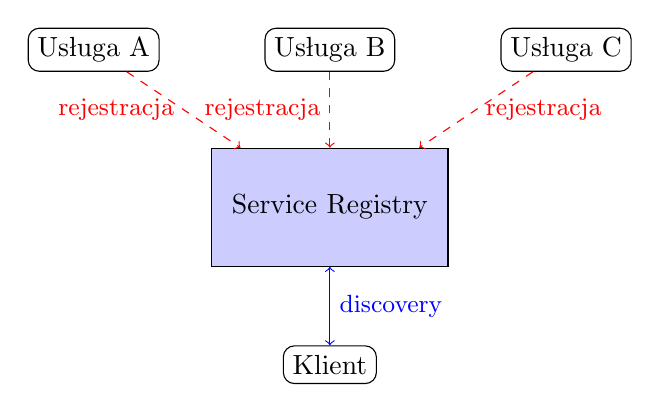
\begin{tikzpicture}
            \node[draw, fill=blue!20, minimum width=3cm, minimum height=1.5cm] (registry) at (0,0) {Service Registry};
            \node[draw, rounded corners] (service1) at (-3,2) {Usługa A};
            \node[draw, rounded corners] (service2) at (0,2) {Usługa B};
            \node[draw, rounded corners] (service3) at (3,2) {Usługa C};
            \node[draw, rounded corners] (client) at (0,-2) {Klient};
            
            \draw[->, dashed, color=red] (service1) -- (registry) node[midway, left] {\small rejestracja};
            \draw[->, dashed, color=red] (service2) -- (registry) node[midway, left] {\small rejestracja};
            \draw[->, dashed, color=red] (service3) -- (registry) node[midway, right] {\small rejestracja};
            \draw[<->, color=blue] (client) -- (registry) node[midway, right] {\small discovery};
        \end{tikzpicture}
    \end{center}
    
    \begin{itemize}
        \item Popularne implementacje:
        \begin{itemize}
            \item Consul
            \item etcd
            \item Zookeeper
            \item Eureka
        \end{itemize}
    \end{itemize}
\end{frame}

\begin{frame}{Typy Service Discovery}
    \begin{columns}
        \begin{column}{0.5\textwidth}
            \textbf{Client-Side Discovery}
            \begin{center}
                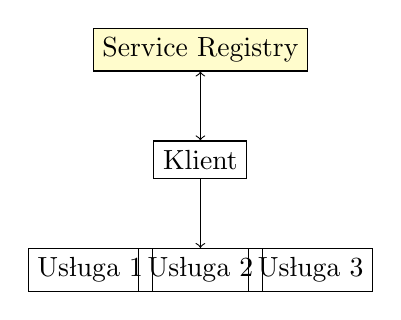
\begin{tikzpicture}[scale=0.7]
                    \node[draw, fill=yellow!20] (reg) at (0,2) {Service Registry};
                    \node[draw] (client) at (0,0) {Klient};
                    \node[draw] (serv1) at (-2,-2) {Usługa 1};
                    \node[draw] (serv2) at (0,-2) {Usługa 2};
                    \node[draw] (serv3) at (2,-2) {Usługa 3};
                    
                    \draw[<->] (client) -- (reg);
                    \draw[->] (client) -- (serv2);
                \end{tikzpicture}
            \end{center}
            \begin{itemize}
                \item Klient odpowiedzialny za określenie lokalizacji
                \item Klient musi implementować logikę discovery
                \item Pełna kontrola nad wyborem instancji
            \end{itemize}
        \end{column}
        
        \begin{column}{0.5\textwidth}
            \textbf{Server-Side Discovery}
            \begin{center}
                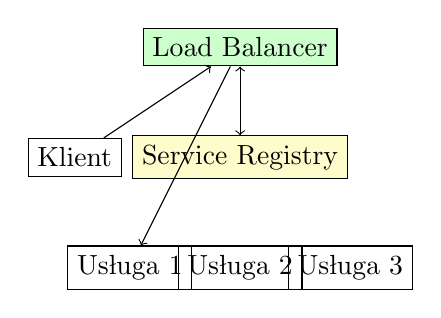
\begin{tikzpicture}[scale=0.7]
                    \node[draw, fill=yellow!20] (reg) at (0,0) {Service Registry};
                    \node[draw] (client) at (-3,0) {Klient};
                    \node[draw, fill=green!20] (lb) at (0,2) {Load Balancer};
                    \node[draw] (serv1) at (-2,-2) {Usługa 1};
                    \node[draw] (serv2) at (0,-2) {Usługa 2};
                    \node[draw] (serv3) at (2,-2) {Usługa 3};
                    
                    \draw[<->] (lb) -- (reg);
                    \draw[->] (client) -- (lb);
                    \draw[->] (lb) -- (serv1);
                \end{tikzpicture}
            \end{center}
            \begin{itemize}
                \item Klient kontaktuje się z load balancerem
                \item Load balancer komunikuje się z rejestrem
                \item Prostszy kod klienta
                \item Dodatkowy komponent (load balancer)
            \end{itemize}
        \end{column}
    \end{columns}
\end{frame}

\section{Kluczowe pojęcia}

\begin{frame}{Opóźnienie (Latency)}
    \begin{block}{Definicja}
        Czas potrzebny na przesłanie wiadomości z jednego węzła systemu do drugiego.
    \end{block}
    
    \begin{itemize}
        \item Czynniki wpływające na opóźnienie:
        \begin{itemize}
            \item Odległość geograficzna między węzłami
            \item Przepustowość sieci
            \item Obciążenie sieci
            \item Czas przetwarzania po stronie serwera
        \end{itemize}
        \vspace{0.3cm}
        \item Znaczenie:
        \begin{itemize}
            \item Krytyczny parametr wydajności
            \item Szczególnie istotny w systemach czasu rzeczywistego
            \item Wpływa na doświadczenie użytkownika
        \end{itemize}
    \end{itemize}
\end{frame}

\begin{frame}{Przepustowość (Throughput)}
    \begin{block}{Definicja}
        Ilość danych, które system może przetworzyć w jednostce czasu.
    \end{block}
    
    \begin{itemize}
        \item Ograniczenia przepustowości:
        \begin{itemize}
            \item Przepustowość fizycznych połączeń sieciowych
            \item Wydajność serwerów i innych komponentów sprzętowych
            \item Efektywność algorytmów i implementacji oprogramowania
        \end{itemize}
        \vspace{0.3cm}
        \item Zwiększanie przepustowości:
        \begin{itemize}
            \item Skalowanie horyzontalne (dodawanie więcej instancji)
            \item Optymalizacja kodu i algorytmów
            \item Techniki cache'owania
            \item Równoważenie obciążenia
        \end{itemize}
    \end{itemize}
\end{frame}

\begin{frame}{High Availability (Wysoka dostępność)}
    \begin{block}{Definicja}
        Zdolność systemu do działania przez długi czas bez przerw.
    \end{block}
    
    \begin{itemize}
        \item Wyrażana jako procent czasu dostępności:
        \begin{itemize}
            \item 99,9\% (three nines) = 8,76 godziny przestoju/rok
            \item 99,99\% (four nines) = 52,56 minuty przestoju/rok
            \item 99,999\% (five nines) = 5,26 minuty przestoju/rok
        \end{itemize}
        \vspace{0.3cm}
        \item Mechanizmy zapewniające wysoką dostępność:
        \begin{itemize}
            \item Redundancja - duplikacja krytycznych komponentów
            \item Replikacja danych - kopie danych na wielu serwerach
            \item Równoważenie obciążenia - dystrybucja ruchu
            \item Automatyczne odzyskiwanie - przywracanie po awarii
            \item Mechanizmy failover - przełączanie na systemy zapasowe
        \end{itemize}
    \end{itemize}
\end{frame}

\section{Studium przypadku}

\begin{frame}{Studium przypadku - system rozproszony w organizacji finansowej}
    \begin{block}{Kontekst i wymagania}
        Organizacja finansowa potrzebuje systemu, który spełnia następujące wymagania:
        \begin{itemize}
            \item Wysoka dostępność (99,999\%)
            \item Skalowalność - miliony transakcji dziennie
            \item Bezpieczeństwo - najwyższy poziom ochrony danych
            \item Elastyczność - szybkie wprowadzanie nowych funkcji
        \end{itemize}
    \end{block}
\end{frame}

\begin{frame}{Architektura systemu}
    \begin{center}
        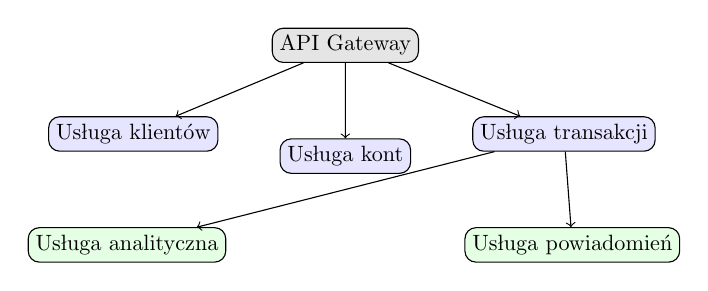
\begin{tikzpicture}[node distance=1.2cm, scale=0.8, transform shape]
            \node[draw, rounded corners, fill=gray!20] (api) {API Gateway};
            \node[draw, rounded corners, fill=blue!10, below left=of api] (clients) {Usługa klientów};
            \node[draw, rounded corners, fill=blue!10, below=of api] (accounts) {Usługa kont};
            \node[draw, rounded corners, fill=blue!10, below right=of api] (transactions) {Usługa transakcji};
            \node[draw, rounded corners, fill=green!10, below left=of accounts] (analytics) {Usługa analityczna};
            \node[draw, rounded corners, fill=green!10, below right=of accounts] (notifications) {Usługa powiadomień};
            
            \draw[->] (api) -- (clients);
            \draw[->] (api) -- (accounts);
            \draw[->] (api) -- (transactions);
            \draw[->] (transactions) -- (analytics);
            \draw[->] (transactions) -- (notifications);
        \end{tikzpicture}
    \end{center}
    
    \begin{itemize}
        \item Architektura mikrousług:
        \begin{itemize}
            \item Każda usługa jest odpowiedzialna za konkretną domenę biznesową
            \item Usługi mogą być rozwijane, testowane i wdrażane niezależnie
            \item Możliwość skalowania poszczególnych usług
        \end{itemize}
    \end{itemize}
\end{frame}

\begin{frame}{Wzorce komunikacji w systemie}
    \begin{itemize}
        \item \textbf{HTTP/REST}
        \begin{itemize}
            \item Dla komunikacji między aplikacjami klientów a API Gateway
            \item Łatwość implementacji i szeroka obsługa przeglądarek
        \end{itemize}
        \vspace{0.3cm}
        \item \textbf{gRPC}
        \begin{itemize}
            \item Dla komunikacji między mikrousługami
            \item Wydajność i ścisła specyfikacja kontraktu
        \end{itemize}
        \vspace{0.3cm}
        \item \textbf{Message Queues}
        \begin{itemize}
            \item Dla operacji asynchronicznych (przetwarzanie transakcji, raporty)
            \item Model hybrydowy, łączący cechy point-to-point i pub/sub
        \end{itemize}
    \end{itemize}
\end{frame}

\begin{frame}{Service Discovery i wysoka dostępność}
    \begin{columns}
        \begin{column}{0.5\textwidth}
            \textbf{Service Discovery}
            \begin{itemize}
                \item Server-side discovery
                \item Usługi rejestrują się w service registry
                \item Load balancer kieruje ruch do odpowiednich instancji
                \item Regularne health checks
            \end{itemize}
        \end{column}
        
        \begin{column}{0.5\textwidth}
            \textbf{Wysoka dostępność}
            \begin{itemize}
                \item Redundancja - wiele instancji usług
                \item Automatyczne skalowanie
                \item Circuit breaker - zapobieganie kaskadowym awariom
                \item Monitorowanie i alerting
            \end{itemize}
        \end{column}
    \end{columns}
    
    \begin{block}{Kluczowa zaleta}
        Awaria jednego komponentu nie wpływa na działanie całego systemu.
    \end{block}
\end{frame}

\section{Podsumowanie}

\begin{frame}{Podsumowanie}
    \begin{itemize}
        \item \textbf{Warstwy systemu}
        \begin{itemize}
            \item Prezentacji, logiki biznesowej i danych
            \item Organizacja systemu i izolacja odpowiedzialności
        \end{itemize}
        \vspace{0.3cm}
        \item \textbf{Wzorce komunikacji}
        \begin{itemize}
            \item Synchroniczne (HTTP/REST, gRPC)
            \item Asynchroniczne (kolejki, publish/subscribe)
        \end{itemize}
        \vspace{0.3cm}
        \item \textbf{Service registry i discovery}
        \begin{itemize}
            \item Dynamiczne odnajdywanie usług
            \item Client-side i server-side discovery
        \end{itemize}
        \vspace{0.3cm}
        \item \textbf{Kluczowe pojęcia}
        \begin{itemize}
            \item Opóźnienie, przepustowość, wysoka dostępność
        \end{itemize}
    \end{itemize}
\end{frame}

\begin{frame}{Źródła i literatura}
    \begin{thebibliography}{9}
        \bibitem{tanenbaum} Tanenbaum A.S., Van Steen M., \emph{Distributed Systems: Principles and Paradigms}, Pearson Prentice Hall, 2006.
        
        \bibitem{newman} Newman S., \emph{Building Microservices}, O'Reilly Media, 2015.
        
        \bibitem{richardson} Richardson C., \emph{Microservices Patterns}, Manning Publications, 2018.
        
        \bibitem{fowler} Fowler M., \emph{Patterns of Enterprise Application Architecture}, Addison-Wesley, 2002.
        
        \bibitem{burns} Burns B., \emph{Designing Distributed Systems}, O'Reilly Media, 2018.
    \end{thebibliography}
\end{frame}

\begin{frame}
    \centering
    \Huge Dziękuję za uwagę!
    
    \vspace{1cm}
    
    \Large Pytania?
\end{frame}

\end{document}
